\pagebreak
\section{Przypadki testowe}
\newcommand{\specialcell}[2][c]{
  \begin{tabular}[#1]{@{}l@{}}#2\end{tabular}}
	
	\graphicspath{{obrazki/}}
	
	\begin{longtable}{ p{.50\textwidth} p{.50\textwidth} }
	
	
	
	\specialcell{
	\textbf{1.} $p_1 = 0.25$  \\
	\textbf{2.} $p_1 = 0.5$ \\
	Rozkład równomierny: \\ 
	$a_1 = 200, b_1 = 300$ \\
	$a_2 = 240, b_2 = 250$ \\
	Rozkład normalny: \\
	$\sigma_1 = 250, \mu_1 = 50$ \\
	$\sigma_2 = 250, \mu_2 = 5$ \\
	Teoretyczne ryzyko Bayesa: \\
	$R_U = 0.1$ \\
	$R_N = 0.08$ \\
	} & \parbox[c]{1cm}{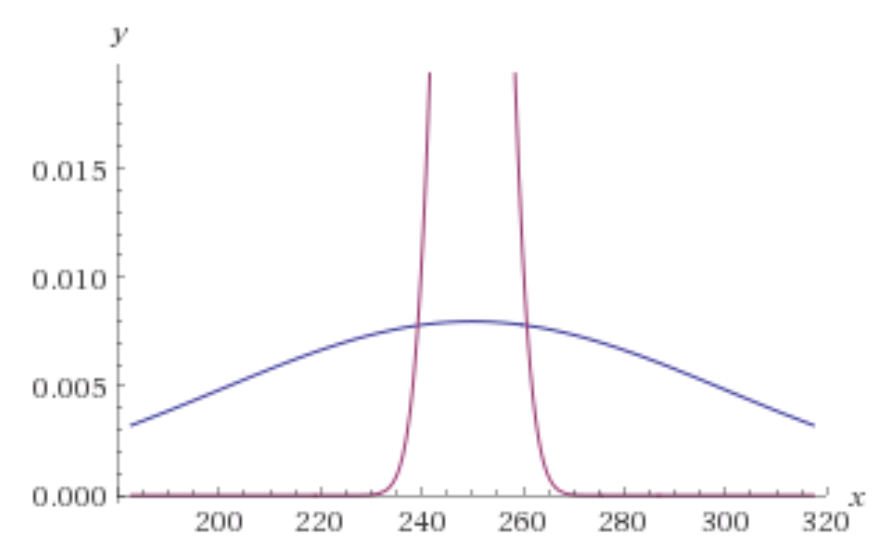
\includegraphics[width=.50\textwidth,trim=0 0 0 -5]{1.png}}\\
	
	\\
	 
	
	\specialcell{
	\textbf{3.} $p_1 = 0.25$  \\
	\textbf{4.} $p_1 = 0.5$ \\
	Rozkład równomierny: \\ 
	$a_1 = 200, b_1 = 300$ \\
	$a_2 = 250, b_2 = 350$ \\
	Rozkład normalny: \\
	$\sigma_1 = 0, \mu_1 = 1$ \\
	$\sigma_2 = 1, \mu_2 = 1$ \\
	Teoretyczne ryzyko Bayesa: \\
	$R_U = 0.5$ \\
	$R_N = 0.246$ \\
	} & \parbox[c]{1cm}{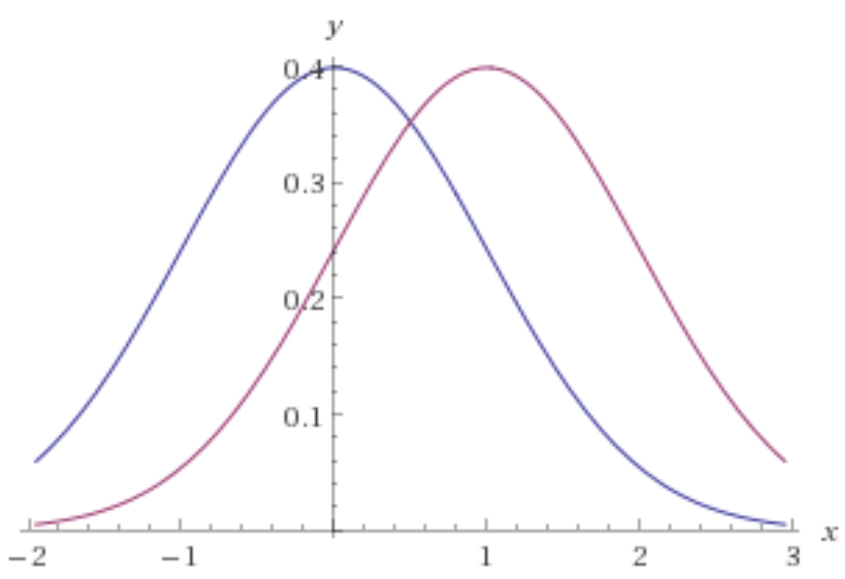
\includegraphics[width=.50\textwidth,trim=0 0 0 -5]{2.png}}\\
	
	\\
	
	\specialcell{
	\textbf{5.} $p_1 = 0.25$  \\
	\textbf{6.} $p_1 = 0.5$ \\
	Rozkład równomierny: \\ 
	$a_1 = 200, b_1 = 300$ \\
	$a_2 = 290, b_2 = 390$ \\
	Rozkład normalny: \\
	$\sigma_1 = 0, \mu_1 = \sqrt{0.2}$ \\
	$\sigma_2 = 1, \mu_2 = \sqrt{0.2}$ \\
	Teoretyczne ryzyko Bayesa: \\
	$R_U = 0.1$ \\
	$R_N = 0.105$ \\
	} & \parbox[c]{1cm}{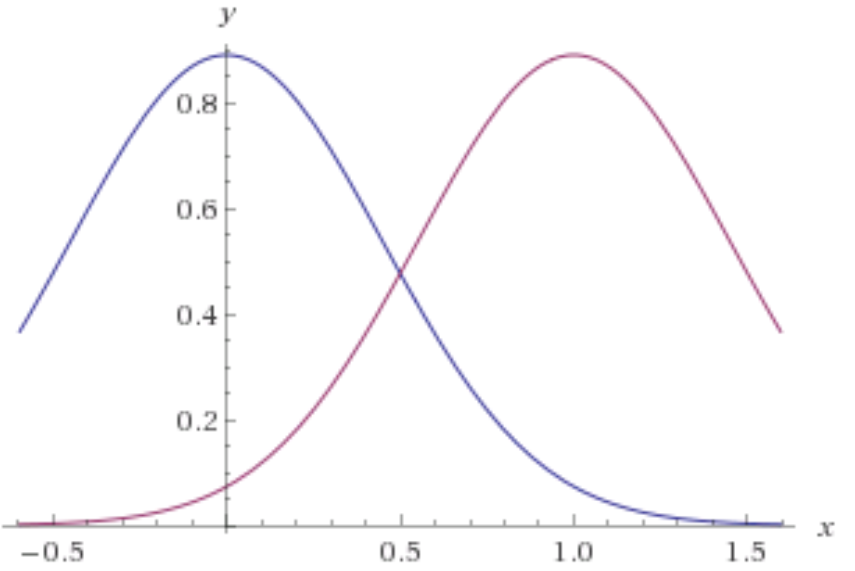
\includegraphics[width=.50\textwidth,trim=0 0 0 -5]{3.png}}\\
	
	\\
	
	\specialcell{
	\textbf{7.} $p_1 = 0.25$  \\
	\textbf{8.} $p_1 = 0.5$ \\
	Rozkład równomierny: \\ 
	$a_1 = 200, b_1 = 300$ \\
	$a_2 = 300, b_2 = 400$ \\
	Rozkład normalny: \\
	$\sigma_1 = 0, \mu_1 = \sqrt{0.5}$ \\
	$\sigma_2 = 5, \mu_2 = \sqrt{0.5}$ \\
	Teoretyczne ryzyko Bayesa: \\
	$R_U = 0.01$ \\
	$R_N = 0.00016$ \\
	} & \parbox[c]{1cm}{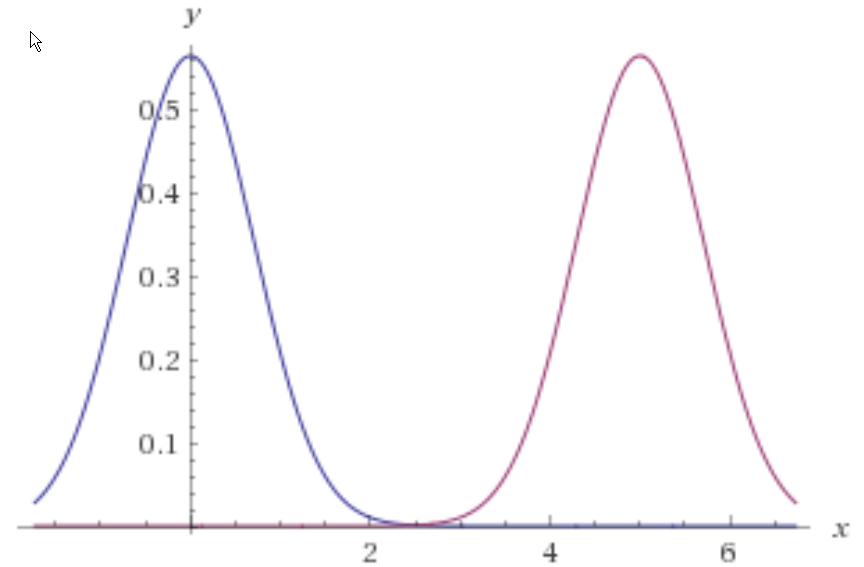
\includegraphics[width=.50\textwidth,trim=0 0 0 -5]{4.png}}\\
	
	\\
	
	\specialcell{
	\textbf{9.} $p_1 = 0.25$  \\
	\textbf{10.} $p_1 = 0.5$ \\
	Rozkład równomierny: \\ 
	$a_1 = 200, b_1 = 300$ \\
	$a_2 = 350, b_2 = 450$ \\
	Rozkład normalny: \\
	$\sigma_1 = 0, \mu_1 = \sqrt{0.5}$ \\
	$\sigma_2 = 7, \mu_2 = \sqrt{0.5}$ \\
	Teoretyczne ryzyko Bayesa: \\
	$R_U = 0$ \\
	$R_N = 3*10^{-7}$ \\
	} & \parbox[c]{1cm}{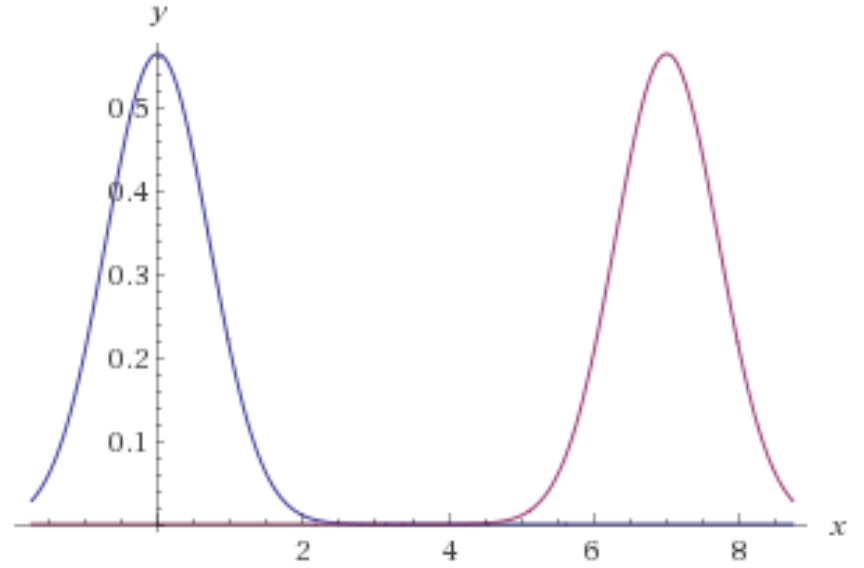
\includegraphics[width=.50\textwidth,trim=0 0 0 -5]{5.png}}\\
	
	
	\end{longtable}